\documentclass[10pt,landscape]{article}
\usepackage[utf8]{inputenc}
\usepackage[margin=0.4in]{geometry}
\usepackage{multicol}
\usepackage{xcolor}
\usepackage{listings}
\usepackage{tikz}
\usetikzlibrary{shapes.geometric, arrows.meta, positioning}

\lstset{
    backgroundcolor=\color{gray!10},
    basicstyle=\ttfamily\tiny,
    breaklines=true,
    frame=single,
    showstringspaces=false
}


\newcommand{\sectionheader}[1]{%
    \vspace{2pt}\noindent\colorbox{blue!15}{\parbox{\dimexpr\linewidth-2\fboxsep}{%
    \textbf{#1}}}\vspace{2pt}%
}

\tikzset{
    myarrow/.style={-{Stealth}},
    box/.style={draw, rectangle, font=\tiny, fill=white, minimum width=1.5cm, minimum height=0.6cm, align=center}
}

\begin{document}
\begin{multicols*}{3}

% --- PAGE 1: SETUP & ESSENTIALS ---
\begin{center}\textbf{\Large CKA CHEATSHEET: PAGE 1}\\\textit{The Command Center}\end{center}

\sectionheader{1. Setup \& Aliases}
\begin{lstlisting}
alias k='kubectl'
alias kgp='k get pods'
alias kgs='k get svc'
export do="--dry-run=client -o yaml"
export now="--force --grace-period=0"
# Vim: :set ts=2 sw=2 et
\end{lstlisting}

\sectionheader{2. Cluster Architecture}
\begin{center}
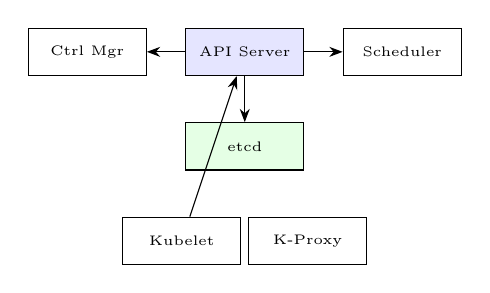
\begin{tikzpicture}[node distance=1.2cm]
    \node (api) [box, fill=blue!10] {API Server};
    \node (etcd) [box, below of=api, fill=green!10] {etcd};
    \node (sched) [box, right of=api, xshift=0.8cm] {Scheduler};
    \node (cm) [box, left of=api, xshift=-0.8cm] {Ctrl Mgr};
    \node (kubelet) [box, below of=etcd, xshift=-0.8cm] {Kubelet};
    \node (proxy) [box, below of=etcd, xshift=0.8cm] {K-Proxy};
    
    \draw [myarrow] (api) -- (etcd);
    \draw [myarrow] (api) -- (sched);
    \draw [myarrow] (api) -- (cm);
    \draw [myarrow] (kubelet) -- (api);
\end{tikzpicture}
\end{center}
\begin{lstlisting}
# Static Pods: /etc/kubernetes/manifests
# Kubelet: /var/lib/kubelet/config.yaml
\end{lstlisting}

\sectionheader{3. Imperative Commands}
\begin{lstlisting}
k run nginx --image=nginx $do
k create deploy web --image=nginx --replicas=3 $do
k expose deploy web --port=80 --type=NodePort
\end{lstlisting}

\columnbreak

% --- PAGE 2: WORKLOADS & SCHEDULING ---
\begin{center}\textbf{\Large CKA CHEATSHEET: PAGE 2}\\\textit{Workloads \& Scheduling}\end{center}

\sectionheader{1. Deployments \& Rollouts}
\begin{center}
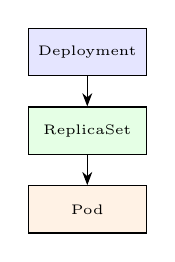
\begin{tikzpicture}[node distance=1.0cm]
    \node (dep) [box, fill=blue!10] {Deployment};
    \node (rs) [box, below of=dep, fill=green!10] {ReplicaSet};
    \node (pod) [box, below of=rs, fill=orange!10] {Pod};
    \draw [myarrow] (dep) -- (rs);
    \draw [myarrow] (rs) -- (pod);
\end{tikzpicture}
\end{center}
\begin{lstlisting}
k rollout status deploy/web
k rollout history deploy/web
k rollout undo deploy/web --to-revision=2
\end{lstlisting}

\sectionheader{2. Scheduling Logic}
\begin{lstlisting}
# NodeSelector
nodeSelector: {disktype: ssd}
# Taints/Tolerations
k taint nodes node1 key=value:NoSchedule
# Node Affinity
affinity:
  nodeAffinity:
    requiredDuringScheduling...
\end{lstlisting}

\sectionheader{3. Admission \& Priority}
\begin{lstlisting}
# PriorityClass
apiVersion: scheduling.k8s.io/v1
kind: PriorityClass
value: 1000000
# Pod: priorityClassName: high-priority
\end{lstlisting}

\sectionheader{3. Resource Management}
\begin{lstlisting}
resources:
  requests: # Scheduling floor
    memory: "64Mi"
    cpu: "250m"
  limits:   # Usage ceiling
    memory: "128Mi"
\end{lstlisting}

\columnbreak

% --- PAGE 3: SERVICES & NETWORKING ---
\begin{center}\textbf{\Large CKA CHEATSHEET: PAGE 3}\\\textit{Services \& Networking}\end{center}

\sectionheader{1. Service Types}
\begin{itemize}
    \item \textbf{ClusterIP}: Internal (Default)
    \item \textbf{NodePort}: Static port on each node (30000-32767)
    \item \textbf{LoadBalancer}: Cloud-provider external IP
\end{itemize}

\sectionheader{2. Ingress \& Gateway API}
\begin{center}
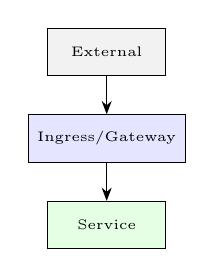
\begin{tikzpicture}[node distance=1.1cm]
    \node (ext) [box, fill=gray!10] {External};
    \node (ing) [box, below of=ext, fill=blue!10] {Ingress/Gateway};
    \node (svc) [box, below of=ing, fill=green!10] {Service};
    \draw [myarrow] (ext) -- (ing);
    \draw [myarrow] (ing) -- (svc);
\end{tikzpicture}
\end{center}
\begin{lstlisting}
# Ingress (pathType: Prefix/Exact)
# Gateway API (HTTPRoute)
apiVersion: gateway.networking.k8s.io/v1
kind: HTTPRoute
spec:
  parentRefs: [{name: my-gateway}]
  rules:
  - backendRefs: [{name: my-svc, port: 80}]
\end{lstlisting}

\sectionheader{3. Network Policies}
\begin{lstlisting}
# Isolation is key. No rule = Deny all.
podSelector: {matchLabels: {app: db}}
ingress:
- from:
  - podSelector: {matchLabels: {app: web}}
\end{lstlisting}

\newpage
% --- PAGE 4: SECURITY ---
\begin{center}\textbf{\Large CKA CHEATSHEET: PAGE 4}\\\textit{Security \& RBAC}\end{center}

\sectionheader{1. RBAC Workflow}
\begin{center}
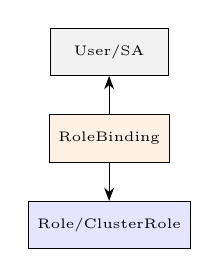
\begin{tikzpicture}[node distance=1.1cm]
    \node (user) [box, fill=gray!10] {User/SA};
    \node (bind) [box, below of=user, fill=orange!10] {RoleBinding};
    \node (role) [box, below of=bind, fill=blue!10] {Role/ClusterRole};
    \draw [myarrow] (bind) -- (user);
    \draw [myarrow] (bind) -- (role);
\end{tikzpicture}
\end{center}
\begin{lstlisting}
# 1. Create Role (Permissions)
k create role reader --verb=get,list --resource=pods
# 2. Bind to ServiceAccount (SA)
k create rolebinding dev-rb --role=reader --serviceaccount=default:sa-1
# Verify: k auth can-i get pods --as system:serviceaccount:default:sa-1
\end{lstlisting}

\sectionheader{2. Service Accounts}
\begin{lstlisting}
k create sa developer-sa
# Assign to Pod:
spec:
  serviceAccountName: developer-sa
\end{lstlisting}

\sectionheader{3. Security Context}
\begin{lstlisting}
securityContext:
  runAsUser: 1000
  capabilities:
    add: ["NET_ADMIN", "SYS_TIME"]
\end{lstlisting}

\columnbreak

% --- PAGE 5: STORAGE ---
\begin{center}\textbf{\Large CKA CHEATSHEET: PAGE 5}\\\textit{Storage \& Volumes}\end{center}

\sectionheader{1. The Storage Handshake}
\begin{center}
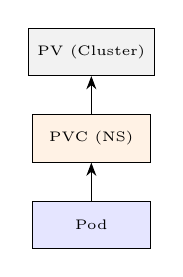
\begin{tikzpicture}[node distance=1.1cm]
    \node (pv) [box, fill=gray!10] {PV (Cluster)};
    \node (pvc) [box, below of=pv, fill=orange!10] {PVC (NS)};
    \node (pod) [box, below of=pvc, fill=blue!10] {Pod};
    \draw [myarrow] (pvc) -- (pv);
    \draw [myarrow] (pod) -- (pvc);
\end{tikzpicture}
\end{center}
\begin{lstlisting}
# PV: capacity, accessModes, hostPath/nfs
# PVC: requests: {storage: 1Gi}
# Dynamic: StorageClass + CSI
k get sc # List StorageClasses
\end{lstlisting}

\sectionheader{2. Volume Mounts}
\begin{lstlisting}
spec:
  containers:
  - volumeMounts:
    - mountPath: "/var/www/html"
      name: my-volume
  volumes:
  - name: my-volume
    persistentVolumeClaim:
      claimName: my-pvc
\end{lstlisting}

\columnbreak

% --- PAGE 6: TROUBLESHOOTING ---
\begin{center}\textbf{\Large CKA CHEATSHEET: PAGE 6}\\\textit{Maintenance \& Troubleshooting}\end{center}

\sectionheader{1. Etcd Backup}
\begin{lstlisting}
export ETCDCTL_API=3
etcdctl --endpoints=... --cacert=... --cert=... --key=... snapshot save /opt/backup.db
\end{lstlisting}

\sectionheader{2. Cluster Upgrade}
\begin{lstlisting}
1. k drain node-1 --ignore-daemonsets
2. apt upgrade kubeadm
3. kubeadm upgrade apply v1.x.y
4. apt upgrade kubelet kubectl
5. k uncordon node-1
\end{lstlisting}

\sectionheader{3. Helm, Kustomize \& Operators}
\begin{lstlisting}
# Helm
helm install app <chart>
# Kustomize
k apply -k <dir>
# CRDs & Operators
k get crd # List CustomResources
k get operators # If OLM installed
\end{lstlisting}

\sectionheader{4. Troubleshooting Flow}
\begin{center}
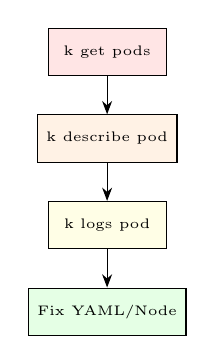
\begin{tikzpicture}[node distance=1.1cm]
    \node (p1) [box, fill=red!10] {k get pods};
    \node (p2) [box, below of=p1, fill=orange!10] {k describe pod};
    \node (p3) [box, below of=p2, fill=yellow!10] {k logs pod};
    \node (p4) [box, below of=p3, fill=green!10] {Fix YAML/Node};
    \draw [myarrow] (p1) -- (p2);
    \draw [myarrow] (p2) -- (p3);
    \draw [myarrow] (p3) -- (p4);
\end{tikzpicture}
\end{center}
\begin{lstlisting}
# Node: systemctl status kubelet
# Logs: journalctl -u kubelet -f
\end{lstlisting}

\end{multicols*}
\end{document}